\documentclass[10pt]{beamer}
\usepackage{etex}
\usetheme[
%%% options passed to the outer theme
%    progressstyle=fixedCircCnt,   %either fixedCircCnt, movCircCnt, or corner
%    rotationcw,          % change the rotation direction from counter-clockwise to clockwise
%    shownavsym          % show the navigation symbols
  ]{AAUsimple}

% If you want to change the colors of the various elements in the theme, edit and uncomment the following lines
% Change the bar and sidebar colors:
%\setbeamercolor{AAUsimple}{fg=green!20,bg=green}
%\setbeamercolor{sidebar}{bg=red!20}
% Change the color of the structural elements:
%\setbeamercolor{structure}{fg=red}
% Change the frame title text color:
%\setbeamercolor{frametitle}{fg=blue}
% Change the normal text color background:
%\setbeamercolor{normal text}{fg=black,bg=gray!10}
% ... and you can of course change a lot more - see the beamer user manual.

\usepackage[utf8]{inputenc}
\usepackage[english]{babel}
\usepackage[T1]{fontenc}
% Or whatever. Note that the encoding and the font should match. If T1
% does not look nice, try deleting the line with the fontenc.
\usepackage{helvet}
\usepackage{xcolor}

%use for graphics
\usepackage{calc}
\usepackage{ifthen}
\usepackage{amsmath,amsfonts,amssymb,amsthm}
\usepackage{mathtools}
\usepackage{todonotes}
\usepackage{listings}
\usepackage{tikz}
\usetikzlibrary{arrows, automata, positioning}
\DeclarePairedDelimiter{\ceil}{\lceil}{\rceil}
\DeclarePairedDelimiter{\floor}{\lfloor}{\rfloor}
\DeclarePairedDelimiter{\tuple}{\langle}{\rangle}
\newcommand{\darrow}{\, \downarrow \!\!}
\newcommand{\uarrow}{\, \uparrow \!\!}

%other package for graphics

%\usepackage{pstricks}
%\usepackage{pstricks-add}

%\usepackage{pst-plot}
\usepackage{xcolor,colortbl}

\newcommand{\mc}[2]{\multicolumn{#1}{c}{#2}}
\definecolor{Gray}{gray}{0.85}

\newcolumntype{a}{>{\columncolor{Gray}}c}
\newcolumntype{b}{>{\columncolor{white}}c}

% command for slices graphic
\newcommand{\slice}[4]{
  \pgfmathparse{0.5*#1+0.5*#2}
  \let\midangle\pgfmathresult

  % slice
  \draw[thick,fill=black!10] (0,0) -- (#1:1) arc (#1:#2:1) -- cycle;

  % outer label
  \node[label=\midangle:#4] at (\midangle:1) {};

  % inner label
  \pgfmathparse{min((#2-#1-10)/110*(-0.3),0)}
  \let\temp\pgfmathresult
  \pgfmathparse{max(\temp,-0.5) + 0.8}
  \let\innerpos\pgfmathresult
  \node at (\midangle:\innerpos) {#3};
}
% colored hyperlinks
\newcommand{\chref}[2]{%
  \href{#1}{{\usebeamercolor[bg]{AAUsimple}#2}}%
}

% Todo commands

\newcommand{\todoin}[2][]{\todo[inline, #1]{#2}}
\newcommand{\fixme}[2][]{\todo[color=yellow!40, #1]{#2}}
\newcommand{\fixmein}[2][]{\todo[inline, color=yellow!40, #1]{#2}}

\definecolor{pblue}{rgb}{0.13,0.13,0.65}
\definecolor{pgreen}{rgb}{0,0.5,0}
\definecolor{pred}{rgb}{0.9,0,0}
\definecolor{porange}{rgb}{0.59,0.29,0}
\definecolor{pgrey}{rgb}{0.34,0.35,0.38}

\lstset{
  language=Java,
  showspaces=false,
  tabsize=2,
  numbers=none,
  showtabs=false,
  breaklines=true,
  showstringspaces=false,
  breakatwhitespace=true,
  commentstyle=\color{pgrey},
  keywordstyle=\color{porange},
  stringstyle=\color{pgreen},
  basicstyle=\small\ubuntumono,
  frame=leftline,
  framesep=5pt,
  framerule=1pt,
  xleftmargin=8pt,
  rulecolor=\color{pblue},
  % moredelim=[il][\textcolor{pgrey}]{$ $},
  % moredelim=[is][\textcolor{pgrey}]{\%\%}{\%\%}
}

\title{Integration of antichain algorithms \\ in automata library}  % could also be a conference name
%\subtitle{Master Thesis in Computer Science}

\date{September 6, 2019}

\author{
  Hakim \textsc{Boulahya}
}

% - Give the names in the same order as they appear in the paper.
% - Use the \inst{?} command only if the authors have different
%   affiliation. See the beamer manual for an example

\institute[
%  {\includegraphics[scale=0.2]{aau_segl}}\\ %insert a company, department or university logo
  Faculty of Science
  Université Libre de Bruxelles
  Belgium
] % optional - is placed in the bottom of the sidebar on every slide
{% is placed on the bottom of the title page
    supervised by \\
    Emmanuel Filiot and
    Guillermo A. Pérez \\\

  %Département d'Informatique \\
  %Université Libre de Bruxelles \\
  %Belgium

  %there must be an empty line above this line - otherwise some unwanted space is added between the university and the country (I do not know why;( )
}

% specify a logo on the titlepage (you can specify additional logos an include them in
% institute command below
\pgfdeclareimage[height=1.5cm]{titlepagelogo}{img/logoULB} % placed on the title page
\titlegraphic{% is placed on the bottom of the title page
  \pgfuseimage{titlepagelogo}
%  \hspace{1cm}\pgfuseimage{titlepagelogo2}
}
\definecolor{firstcolor}{RGB}{0, 76, 146}
\definecolor{secondcolor}{RGB}{43,46,62}
\definecolor{thirdcolor}{RGB}{180,200,212}

\begin{document}
% the titlepage
{\aauwavesbg%
\begin{frame}[plain,noframenumbering] % the plain option removes the header from the title page
  \titlepage
\end{frame}}
%%%%%%%%%%%%%%%%
%%%%%%%%%%%%%%%%

\section{Introduction}

\begin{frame}{Motivations}{}
    \begin{block}{Scenario}
      \begin{itemize}
        \item A developer wants to implement automata antichain algorithms
        \item How to implement antichains ?
        \item Which tools to use for the automata representation ?
      \end{itemize}
    \end{block}
    \begin{block}{Motivations}
        \begin{itemize}
            \item There exists libraries to use antichains, but not easy to integrate when using automata
            \item Having antichains in automata library \textit{seems} to be needed
        \end{itemize}
    \end{block}
    \begin{center}
        \textbf{Ease the implementation of antichain-based algorithms \\ for developers}
    \end{center}
\end{frame}

\begin{frame}[fragile]{Contributions}
  \begin{block}{Objectives}
      \begin{itemize}
          \item The goal of the thesis was to define a use case algorithm using antichains: \\ \textbf{Language universality check $L(A) \stackrel{?}{=} \Sigma^*$ using antichains}
          \item Then implement it in an automata library: \\ \textbf{Owl: $\omega$-automata library}
      \end{itemize}
\\~\\

At the end we should have something like:
      \begin{lstlisting}
owl -I myautomaton.hoa \
hoa --- complete --- universality-check --- string
      \end{lstlisting}
  \end{block}

\end{frame}


\begin{frame}{My contributions}
  \begin{block}{Content}
    \begin{itemize}
      \item \texttt{poset} library, a \texttt{Java} library that provides interfaces to interact with antichains \cite{poset-src}
      \item Use case implementation: algorithm for checking universality of NFA using antichains \cite{antichain-universality}
      \item a \textit{User Guide} (this work) on how to integrate an algorithm in \texttt{Owl} \cite{owl}
    \end{itemize}
    \begin{center}
      \textbf{The main goal is to provide a framework \\ to implement antichain algorithms in automata libraries}
    \end{center}
  \end{block}
\end{frame}

\begin{frame}[fragile]{\texttt{poset} library}

\begin{center}
\texttt{poset} is a \texttt{Java} library providing interfaces for: \\ orders, bounds and antichains
\end{center}

\begin{itemize}
  \item All functions are implemented using the \texttt{FunctionalInterface}: single method class using lambda expressions syntax
  \item Antichains (and closed sets) are implemented using \texttt{Set} interfaces
  \item Interfaces use generic types, and default implementations make use of builtin interfaces: \texttt{Set} for set of elements and \texttt{List} for vectors representation
\end{itemize}

\end{frame}

\begin{frame}[fragile]{\texttt{poset} functions}

\begin{block}{Orders}
    \begin{lstlisting}
interface Order<T> extends BiPredicate<T, T>
    \end{lstlisting}
    \begin{itemize}
      \item With implementations for: $\subseteq$, $\sqsubseteq$ and $\preceq$
    \end{itemize}
\end{block}


\begin{block}{Bounds}
    \begin{lstlisting}
public interface Bound<T>{
  T compute(T a, T b, Order<T> order)
}
    \end{lstlisting}
    \begin{itemize}
      \item With an implementation for the greatest lower bound $a \sqcap b$
    \end{itemize}
\end{block}

\end{frame}

\begin{frame}[fragile]{\texttt{poset} structures}

\begin{block}{Antichains}
    \begin{lstlisting}
interface Antichain<E> extends Set<E>
    \end{lstlisting}
    \begin{itemize}
      \item With one default implementation using a \texttt{LinkedList}\footnote{preferred because it is more needed to add/remove elements than accessing them} to store the incomparable elements
      \item Available methods are the usual for the \texttt{Set} interface (add, remove, contains, etc.) and the union ($\cup$) and intersection ($\cap$) operations
    \end{itemize}
\end{block}

\begin{block}{Closed sets}
  \begin{itemize}
    \item   Mainly antichains where the containment $\in$ is tested against the lower closure $\darrow \ceil{L}$
  \end{itemize}
\end{block}

\end{frame}

\begin{frame}[fragile]{\texttt{poset} examples}

\begin{block}{How it works}

\begin{itemize}
  \item Import the functions
  \begin{lstlisting}
import poset.orders.LEQ
import poset.bounds.GreatestLowerBound
import poset.AntichainList
  \end{lstlisting}
  \item Create them
  \begin{lstlisting}
var leq = new LEQ() // The partial order
var glb = new GreatestLowerBound() // required to compute the intersection
var a1 = new AntichainList<>(leq, glb)
var a2 = new AntichainList<>(leq, glb)
  \end{lstlisting}
  \end{itemize}
\end{block}

\end{frame}

\begin{frame}[fragile]{\texttt{poset} examples}
  \begin{block}{How it works}
    \begin{itemize}
      \item Use it
  \begin{columns}[T]
   \begin{column}{.5\textwidth}
     \begin{lstlisting}
 a1.add(List.of(3, 1))
 //  a1 ==> [[3, 1]]
 a1.add(List.of(2, 2))
 // a1 ==> [[3, 1], [2, 2]]
 a2.add(List.of(0, 2))
 // a2 ==> [[0, 2]]
     \end{lstlisting}
     \end{column}
     \begin{column}{.5\textwidth}
       \begin{lstlisting}
 a1.union(a2)
 // $ ==> [[3, 1], [2, 2]]
 a2.add(List.of(2, 3))
 // a2 ==> [[2, 3]]
 a1.union(a2)
 // $ ==> [[3, 1], [2, 3]]
 a1.intersection(a2)
 // $  ==> [[2, 2]]
       \end{lstlisting}
       \end{column}
 \end{columns}
\end{itemize}

\end{block}

\end{frame}

\begin{frame}{\texttt{Owl} introduction}

\begin{block}{\texttt{Owl} description}

\begin{center}

\texttt{Owl} is a  \textit{"Java tool collection library for $\omega$-words, $\omega$-automata
 and linear temporal logic"}
\end{center}

\begin{itemize}
  \item It can be used either as a command line interface or a library (\texttt{Java} and \texttt{C++} API)
  \item Its a library used mainly for $\omega$-automata and LTL translations
\end{itemize}

\end{block}

\begin{block}{How we use it}

\begin{itemize}
  \item We use \texttt{Owl} as a library to use the automata structures
  \item And we also use \texttt{Owl} as a CLI to run the algorithms
\end{itemize}

\end{block}

\end{frame}

\begin{frame}[fragile]{Integration in \texttt{Owl}}

\begin{block}{How to integrate ?}
\begin{center}
\texttt{Owl} uses a pipelines logic to execute the different modules
\begin{lstlisting}
owl -I myautomaton.hoa \
hoa --- complete --- universality-check --- string
\end{lstlisting}
\end{center}
\end{block}

\begin{itemize}
  \item The goal is to integrate the antichain-based language universality check of an automaton in \texttt{Owl}
  \item It provides a nice interface to integrate any kind of modules that can be chained together to produce a result
\end{itemize}

\end{frame}

\begin{frame}[fragile]{Integration in \texttt{Owl}}

\begin{lstlisting}
owl -I myautomaton.hoa \
hoa --- complete --- universality-check --- string
\end{lstlisting}

\begin{block}{Decomposition of the modules}
\begin{itemize}
  \item \texttt{hoa}: Module reading the input automaton in Hanoi Omega Automata format\footnote{$\omega$-automata have the same structure as NFA so the HOA format can still be used to represent NFAs}
  \item \texttt{complete}: built-in module to complete the input automaton
  \item \texttt{universality-check}: The integrated antichain algorithm
  \item \texttt{string}: the output module, writing \texttt{true} or \texttt{false} in this case
\end{itemize}

\end{block}

\end{frame}

\begin{frame}{Implementation of $L(A) \stackrel{?}{=} \Sigma^*$ }

\begin{block}{}
\begin{itemize}
  \item The \texttt{univerality-check} module is the implementation of the backward antichain algorithm for universality check of an automaton \cite{antichain-universality}
  \item It uses \texttt{Owl} library to interact with automata structures
  \item It uses \texttt{poset} library to build the symbolic representation using antichains
\end{itemize}
\end{block}
\end{frame}

\begin{frame}{Experimental evaluation}

\begin{block}{Comparison}
  \begin{itemize}
    \item The main goal of implementating antichain algorithms is because they perform better than the usual state-of-the-art solutions for the problem
    \item Main comparison for $L(A) \stackrel{?}{=} \Sigma^*$: \textit{antichain-based} vs \textit{subset construction}
  \end{itemize}
\end{block}

\end{frame}

\begin{frame}[fragile]{Experimental evaluation}

\begin{block}{What to compare}
  \begin{enumerate}
    \item \texttt{Owl} (antichain) vs \texttt{VCSN} (subset)
    \begin{itemize}
      \item \texttt{VCSN} is an automata library in \texttt{C++} with \texttt{Python} bindings
      \item It has been chosen for the comparison because it is easy to use and provide lots of
      functions:
      \begin{lstlisting}
a.determinize().complete().complement().is_useless()
      \end{lstlisting}
    \end{itemize}
    \item \texttt{Owl} (antichain) vs \texttt{NuSMV} and \texttt{CUDD} (antichain)
    \begin{itemize}
      \item \texttt{NuSMV} and \texttt{CUDD} are the tools used in the paper  \cite{antichain-universality} that introduced the antichain based algorithm for our use case
    \end{itemize}
  \end{enumerate}
  \begin{itemize}
    \item We want to check that the \texttt{Owl} implementation is better that the subset construction
    \item and is at least as efficient as the one introduced in the original paper
  \end{itemize}
\end{block}
\end{frame}

\begin{frame}{Experimental evaluation}{Methodology}
  \begin{block}{Random automata generation as made in the original paper}
  \begin{itemize}
    \item $\Sigma = \{0, 1\}$
    \item $r$, the transition density
    \item $f = \frac{m}{|Q|}$, the density of accepting states
  \end{itemize}
\end{block}
\end{frame}

\begin{frame}{Experimental evaluation}{Results}
  \begin{columns}[T]
   \begin{column}{.5\textwidth}
       \begin{block}{Owl}
       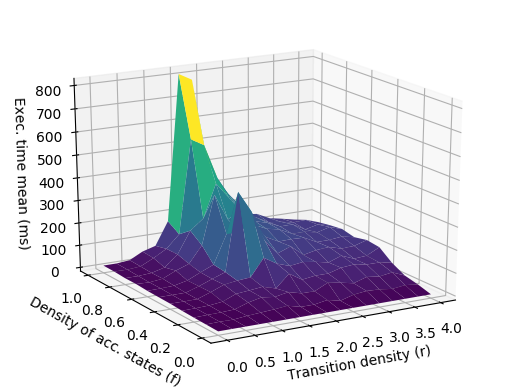
\includegraphics[scale=0.4]{img/defense/this-average-antichain}
       \end{block}
     \end{column}
     \begin{column}{.5\textwidth}
         \begin{block}{VCSN}
            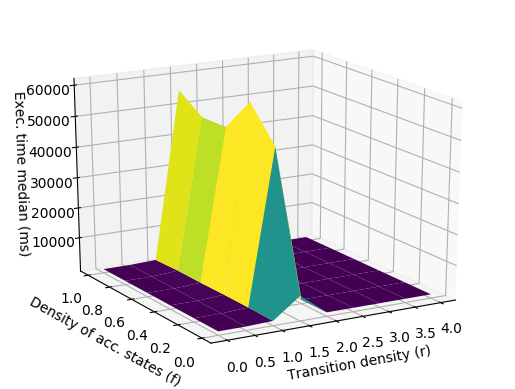
\includegraphics[scale=0.4]{img/defense/vcsn}
         \end{block}
     \end{column}
 \end{columns}
\end{frame}


\begin{frame}{Experimental evaluation}{Results}
  \begin{columns}[T]
   \begin{column}{.5\textwidth}
       \begin{block}{Owl}
       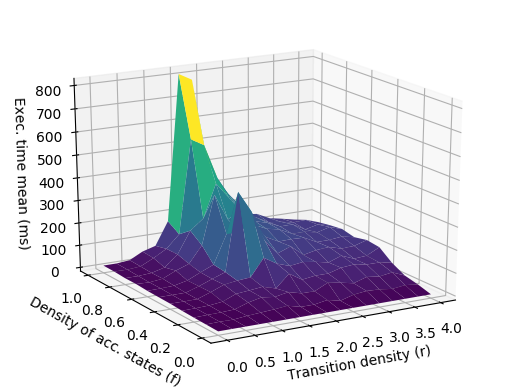
\includegraphics[scale=0.4]{img/defense/this-average-antichain}
       \end{block}
     \end{column}
     \begin{column}{.5\textwidth}
         \begin{block}{NuSMV$^*$}
           \\~\\
            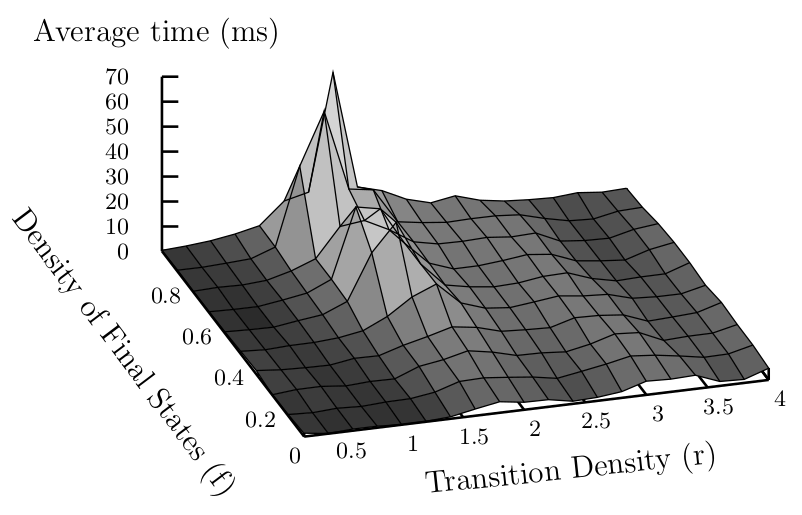
\includegraphics[scale=0.2]{img/defense/original-average-antichain}
         \end{block}
     \end{column}
 \end{columns}
 \\~\\~\\

First results\footnote{Those are the results given in the thesis paper}: 10x slower... Why ? \\~\\
\footnotesize \textbf{*Those results are taken from \cite{antichain-universality} and were not rerun}

\end{frame}

\begin{frame}{Experimental evaluation}{Results}
  \begin{columns}[T]
   \begin{column}{.5\textwidth}
       \begin{block}{Owl}
       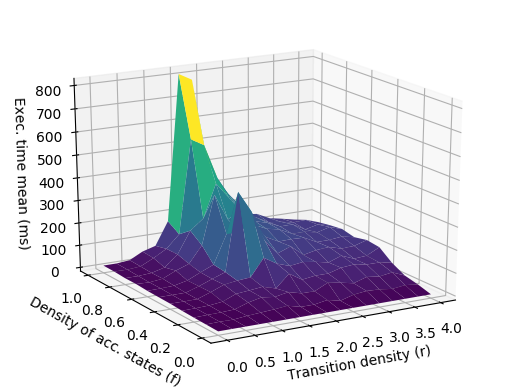
\includegraphics[scale=0.4]{img/defense/this-average-antichain}
       \end{block}
     \end{column}
     \begin{column}{.5\textwidth}
         \begin{block}{Owl with transitions stored in \texttt{HasMap}}
            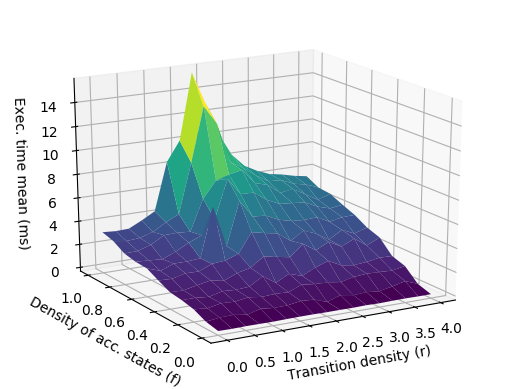
\includegraphics[scale=0.4]{img/defense/with-hashmap-exp5}
         \end{block}
     \end{column}
 \end{columns}
 \\~\\~\\

Successors and predecessors were computed on the fly

\end{frame}

\begin{frame}{Experimental evaluation}{Results}
  \begin{columns}[T]
   \begin{column}{.5\textwidth}
       \begin{block}{Owl}
       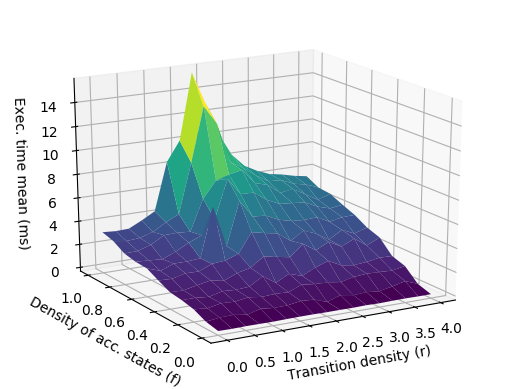
\includegraphics[scale=0.4]{img/defense/with-hashmap-exp5}
       \end{block}
     \end{column}
     \begin{column}{.5\textwidth}
         \begin{block}{NuSMV$^*$}
           \\~\\
            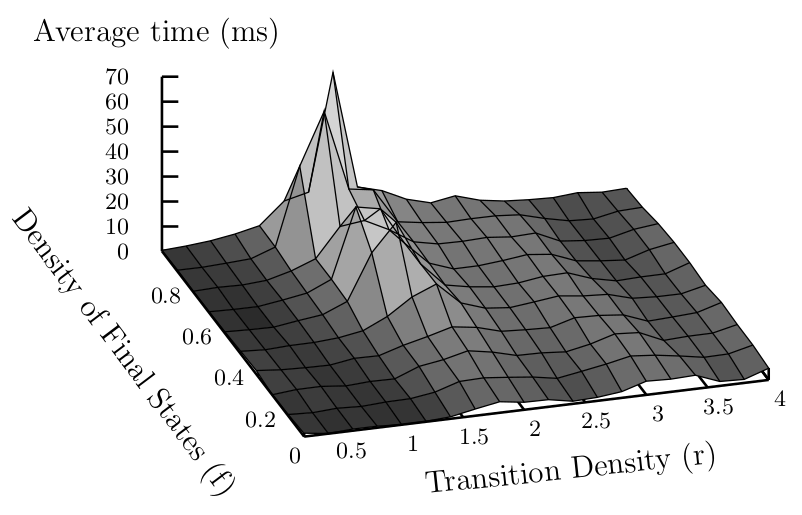
\includegraphics[scale=0.2]{img/defense/original-average-antichain}
         \end{block}
     \end{column}
 \end{columns}
\end{frame}

\def\checkmark{\tikz\fill[scale=0.4](0,.35) -- (.25,0) -- (1,.7) -- (.25,.15) -- cycle;}

\begin{frame}{Conclusion}{}
    \begin{block}{Last year objectives}
        \begin{itemize}
            \item Provide an API and implement it against \texttt{Owl} \checkmark
            \item Provide some implementation for antichains depending
            on the universe of the sets \checkmark
            \item Define the algorithms to test our antichains
            implementation against \checkmark
            \item Study the performance of those implementations \checkmark
        \end{itemize}
    \end{block}
\end{frame}

\begin{frame}{Future work}
  \begin{block}{\texttt{poset} library}
    \begin{itemize}
      \item Improving the default implementation of \texttt{poset} library
      \item Add support for closure operations
    \end{itemize}
  \end{block}
  \begin{block}{Integration}
    \begin{itemize}
      \item A better support of NFA in \texttt{Owl}
      \item \texttt{Owl} can be more user-friendly
      \item Integrate antichains in \texttt{VCSN} since it is more user-friendly
      \item \texttt{Owl} has LTL support, so there are other possibilities of implementation and integration such as \textit{antichain based algorithms for the
synthesis of reactive systems} \cite{bohy-phd}
    \end{itemize}
  \end{block}
\end{frame}

%%%%%%%%%%%%%%%%

{\aauwavesbg
\begin{frame}[allowframebreaks]
    \frametitle{References}
\bibliographystyle{alpha}
\bibliography{thesis}
\end{frame}}

{\aauwavesbg
\begin{frame}[plain,noframenumbering]
  \finalpage{Thanks for listening}
\end{frame}}

\end{document}
